% !TEX root = main.tex
\chapter{RESULTS AND DISCUSSIONS}
\section{General Trends}


In our analysis of MC in the monthly grab samples, the majority of our samples were below the EPA guidance level measured both by \gls{elisa} and \gls{lcmsms}. From our sampled lake sites, Belleville, Brighton, Ford, Hudson, and Wixom Lake had instances of MC concentrations that exceeded the EPA guidance level of 4 $\mu$g/L  (see figure \ref{fig:microcystin}). These instances were primarily high in the month of August. Lake Cadillac, Brighton and Pontiac Lake had concentrations persistently above average amongst all other lakes. In general, MC-RR, MC-LR and MC-LA were the most detected congeners throughout the summer. Brighton Lake had the highest levels of total \gls{lcmsms}, mostly of which is MC-RR with found with a concentrations 8.55 $\mu$g/L in August (see figure \ref{fig:month}). From the analysis of the deployed SPATT measured by \gls{lcmsms}, \gls{mc} results largely varied amongst the different lakes in each month. Observing the congener proportion, MC-LA, MC-LR, and MC-RR were the most frequently detected congener (see \ref{fig:spatter}). Microcystin concentrations from SPATT was mostly detected in Lake Paradise, Intermediate Lake, Lake Cadillac and Wixom Lake. Lake Paradise had the highest amounts of total \gls{mc} with 738 $\frac{\text{ng of MC}}{\text{g of resin x day}}$.  

Of all the sampled lakes, we did not detect cylindrospermonsin in our surveyed lakes from \gls{lcmsms}. Moreover, the QPCR analysis did detect genes responsible for producing cylindrospermonsin (\emph{cyrA}) and saxitoxin (\emph{sxtA}). All sampled lakes had detectable amounts of $log10$\emph{16s rRNA} and $log10$\emph{mcyE} genes (see figure \ref{fig:gene}).  From the \gls{lcmsms} we found one instance of anatoxin-a detected at Brighton lake in August 2017 (2.80 $\mu$g/L of anantoxin-a), which was sampled during a visible bloom. %EPA Graph


\begin{figure}[p]
	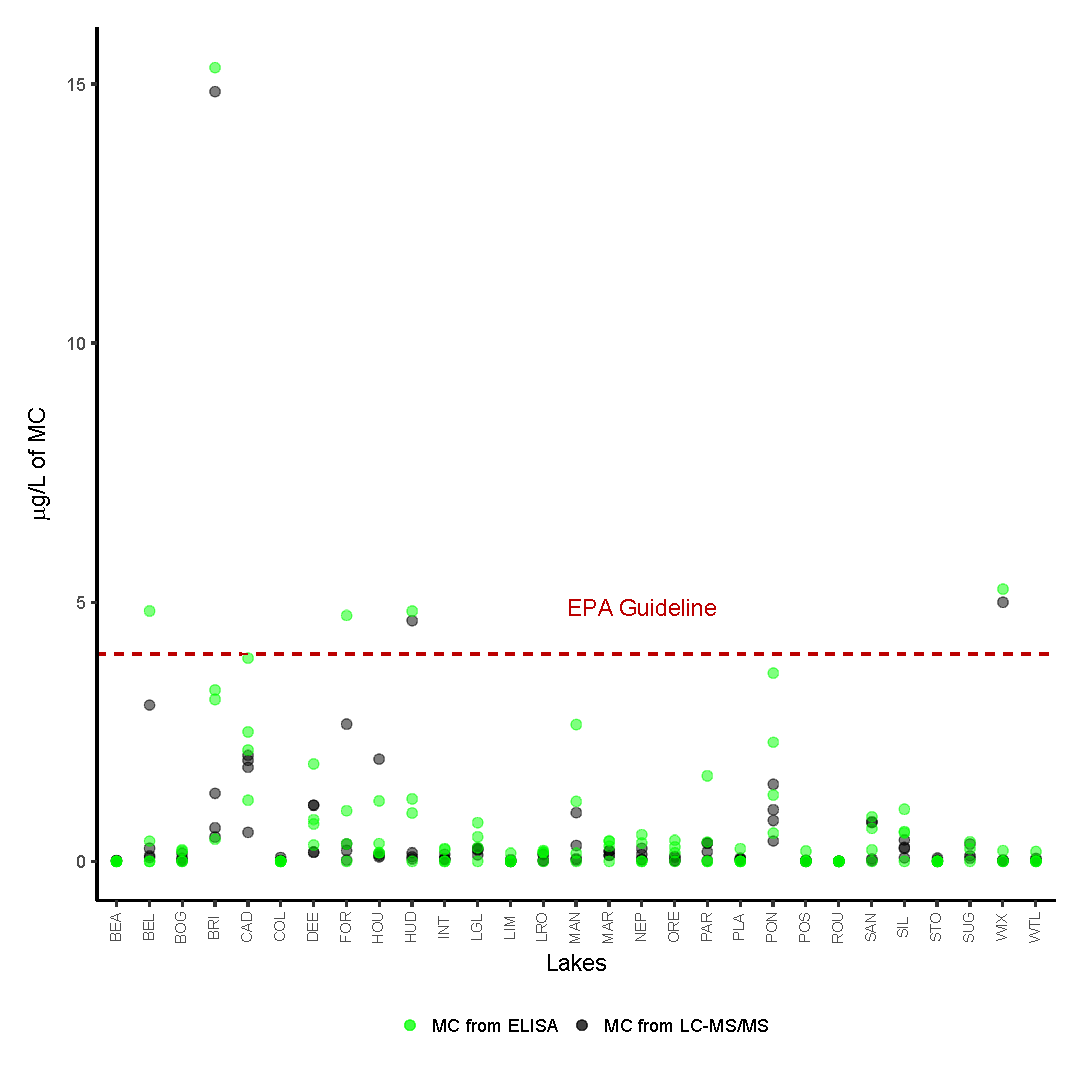
\includegraphics[width=\textwidth]{figures/Microcystin}
	\caption{Total MC with all results from ELISA and LC-MS/MS plotted by each lake.}
	\label{fig:microcystin}
\end{figure}


\begin{figure}[p] 
	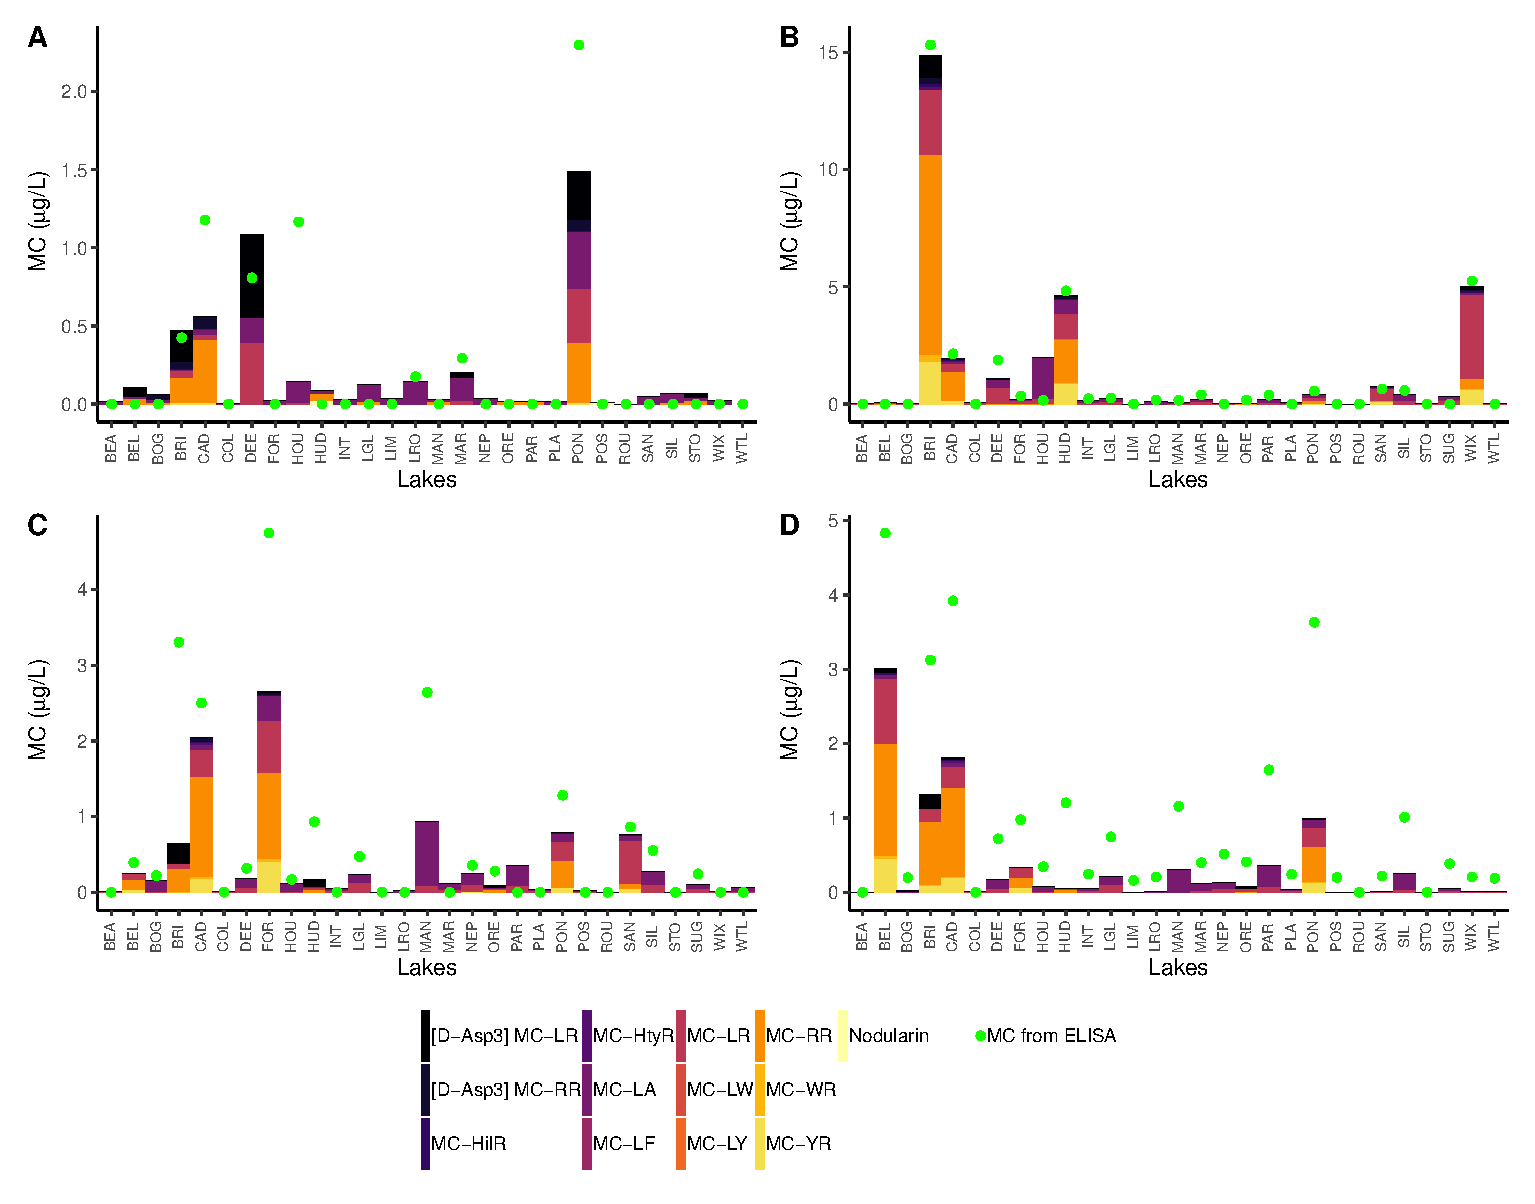
\includegraphics[width=\textwidth]{figures/month}
	\caption{
Barplots of MC and their congeners analyzed by LC-MS/MS from grab sample for each lake for the month of: 
(A) July with missing data from West Twin Lake, 
(B) August,
(C) September, and
(D) October. 
}
	\label{fig:month} 
\end{figure}


\begin{figure}[p] 
	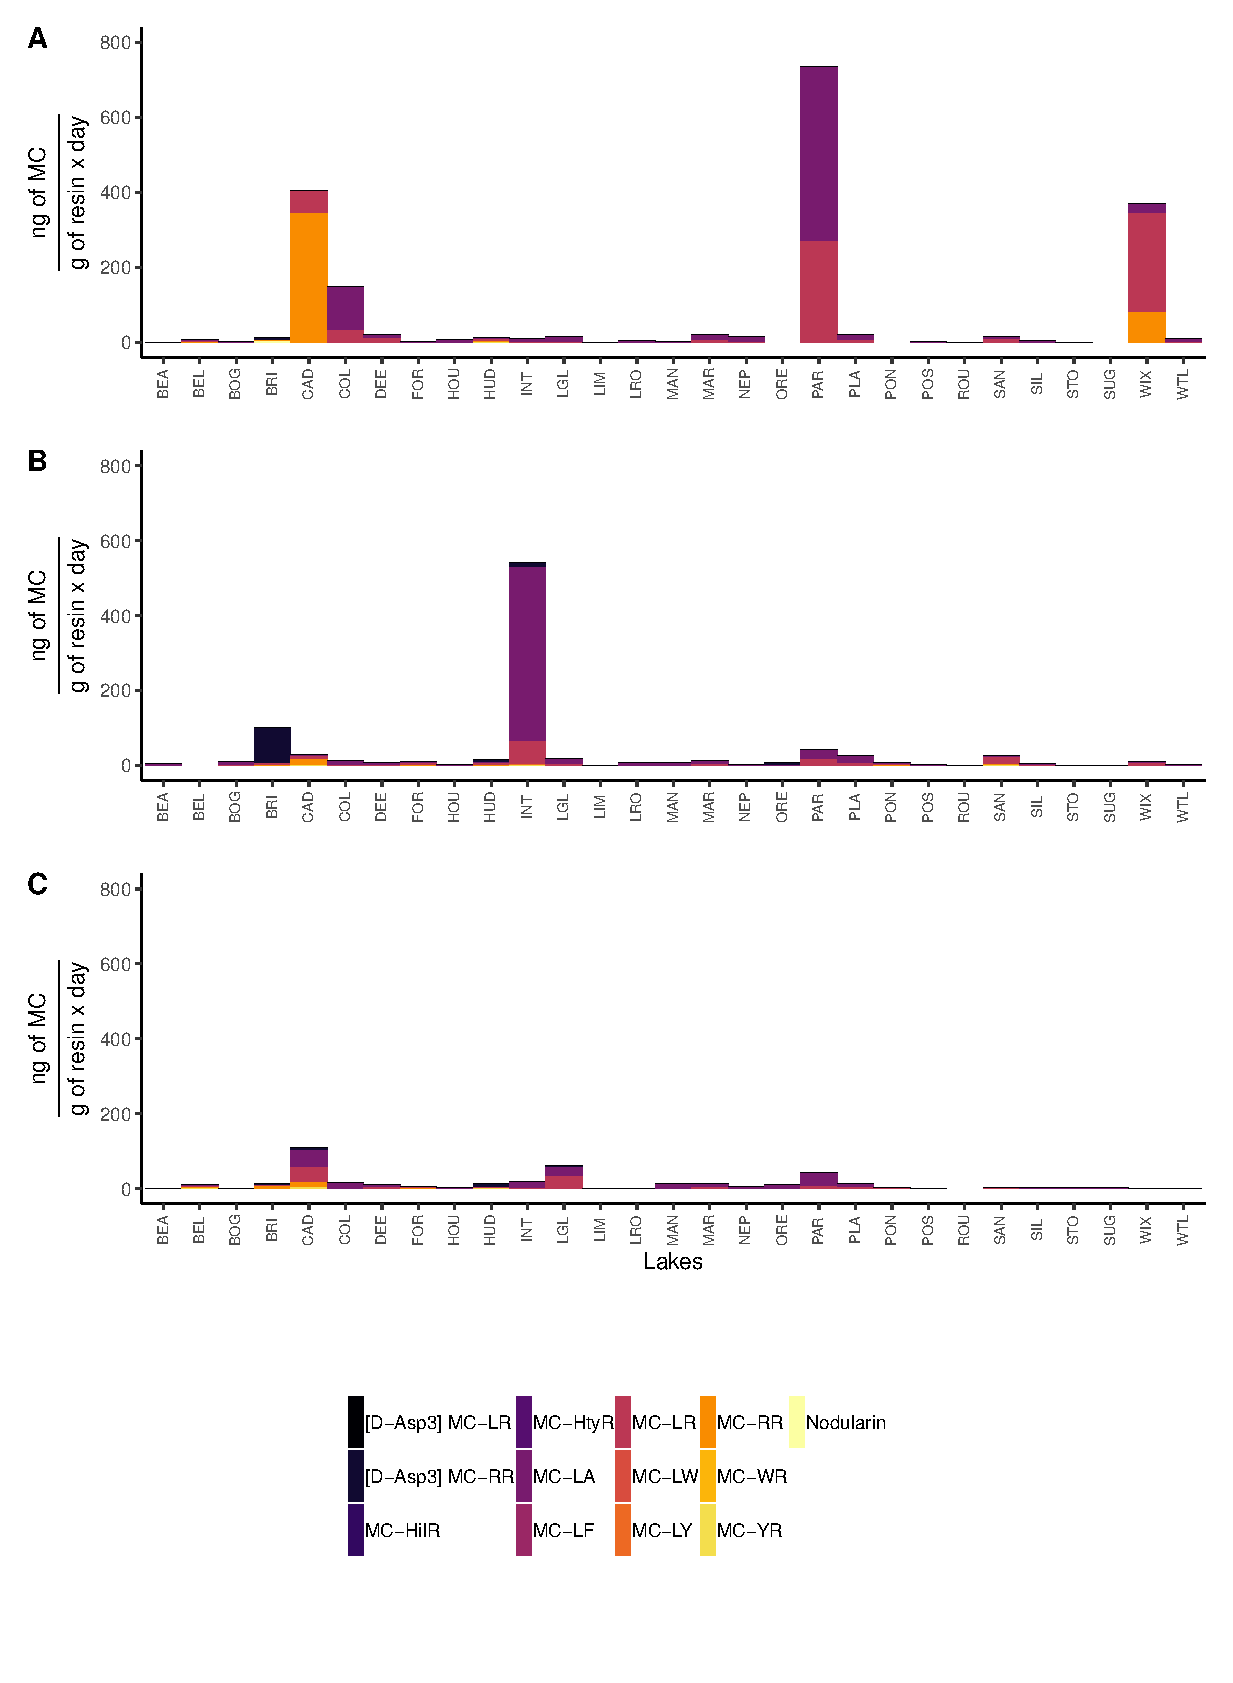
\includegraphics[width=\textwidth]{figures/spatter}
	\vspace*{-15mm}
	\caption{Barplots of MC and their congeners analyzed by LC-MS/MS from deployed SPATT. Concentration is shown for each month of:
(A) July,
(B) August with missing data from Belleville and Pontiac Lake, and
(C) September with missing data from Round Lake.}
	\label{fig:spatter}
\end{figure}


\begin{figure}[p]
	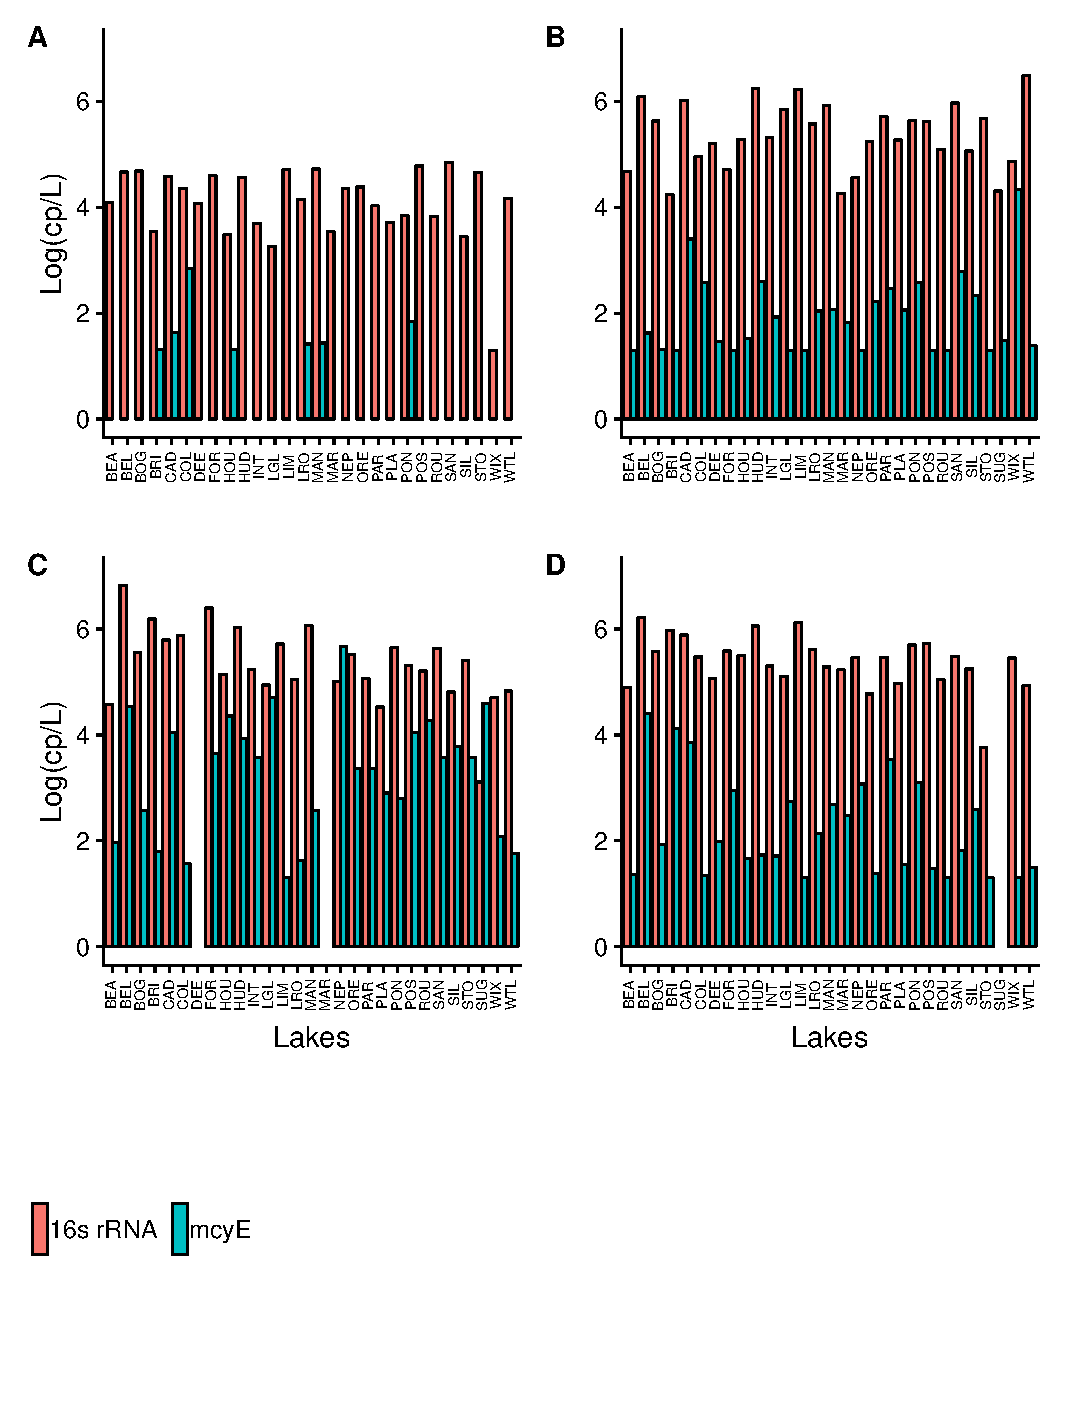
\includegraphics[width=\textwidth]{figures/gene}
	\vspace*{-15mm}
	\caption{
Barplots of \emph{16s rRNA} and \emph{mcyE} results for each month of:
(A) July with results for Brighton, Cadillac, Coldwater, Houghton and  Pontiac as all other lakes have missing data for \emph{mcyE}. 
(B) August,
(C) September with Deer Lake and Lake Margareth with missing data for \emph{16s rRNA} and \emph{mcyE}.
(D) October with missing data from Sugden Lake for both analysis. 
}
	\label{fig:gene}
\end{figure}

%\begin{figure}[!h]
%	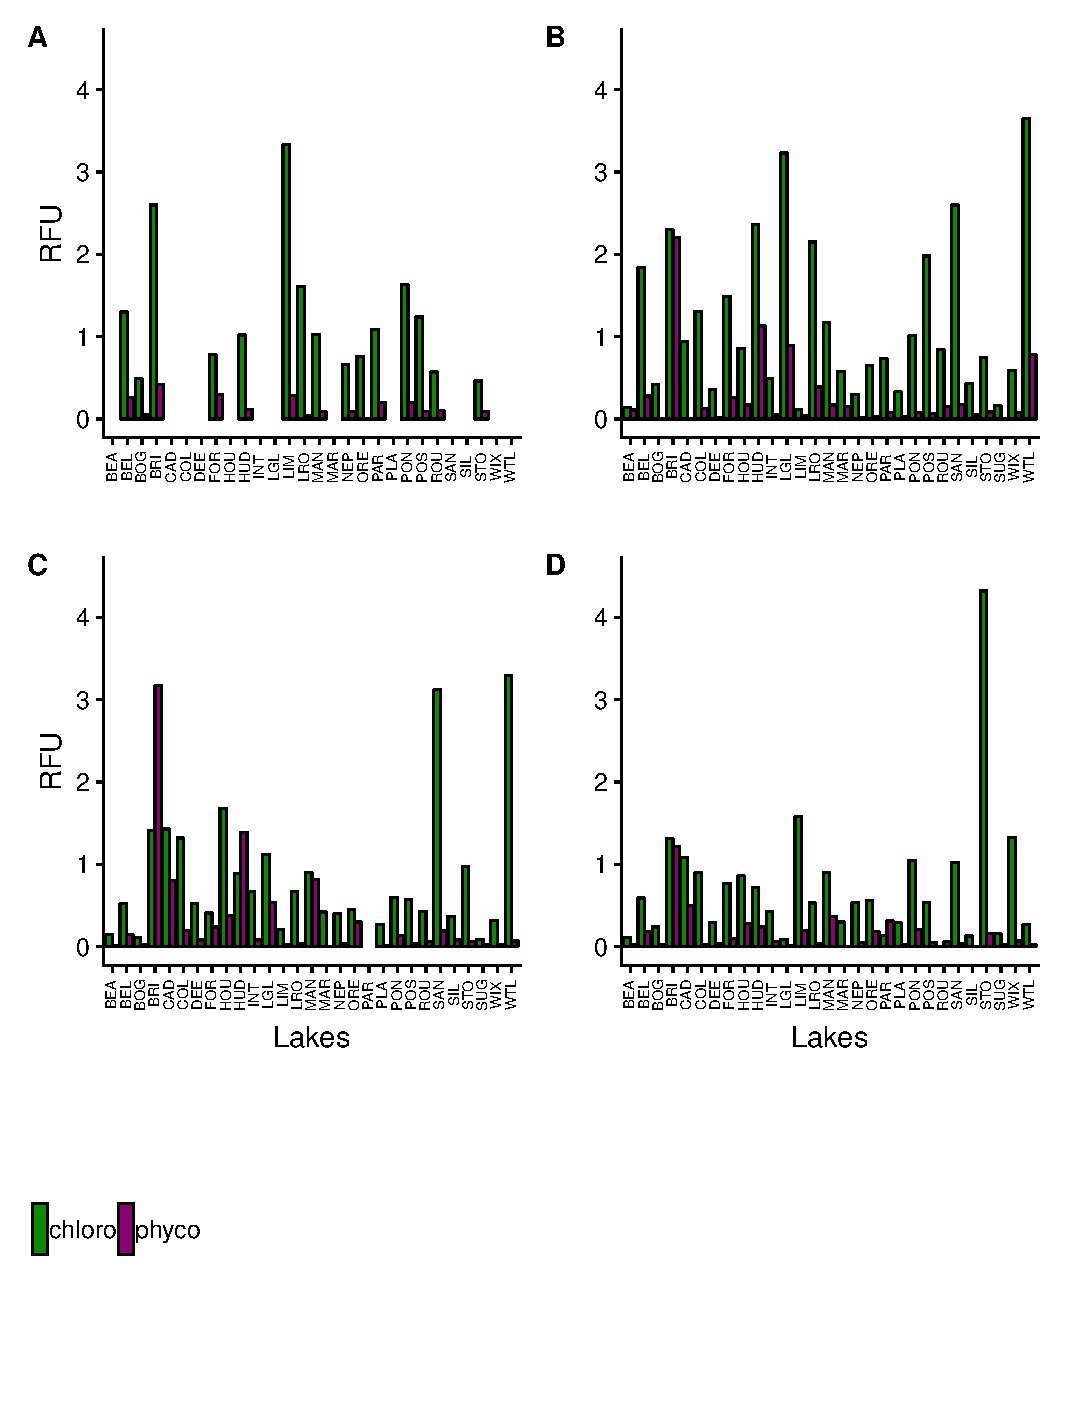
\includegraphics[width=\textwidth]{figures/floro}
%	\vspace*{-15mm}
%	\caption{
%Barplots of chloraphyll and phycocyanin	for each month of:
%(A) July with missing data from Bear, Cadillac, Coldwater, Deer, Houghton, Intermediate, Little Glenn, Lake Margarethe, Platte, Sanford, Silver, Wixom and West Twin Lake. 
%(B) August,
%(C) September with missing data from Lake Paradise, and
%(D) October. 
%}
%	\label{fig:floro}
%\end{figure}


\section{Statistical Modeling}

In our correlation matrix analysis with omitting non-significant correlation ($\alpha>0.05$) we identified few correlated relationships with \gls{lcmsms} (see \ref{matrix}, and see \ref{fig:matrixfull} for the full correlation values). Turbidity, watershed area, orthophosphate and phycocyanin were shown to be correlated with \gls{mc}. Watershed area, water land use, precipitation and forest land use were shown to be negatively correlated with \emph{16s rRNA}. Using best subset analysis found models including turbidity, orthophosphate and pH to be good variables for predicting  $log10$ (\gls{mc}).  
%The best subset analysis is done with the largest subset size of 3 (nvmax=3) and 5 subsets of each size to record (nbest=5) (see figure \ref{fig:subset} and \ref{fig:subset2}).


\begin{sidewaysfigure}[!hp]
	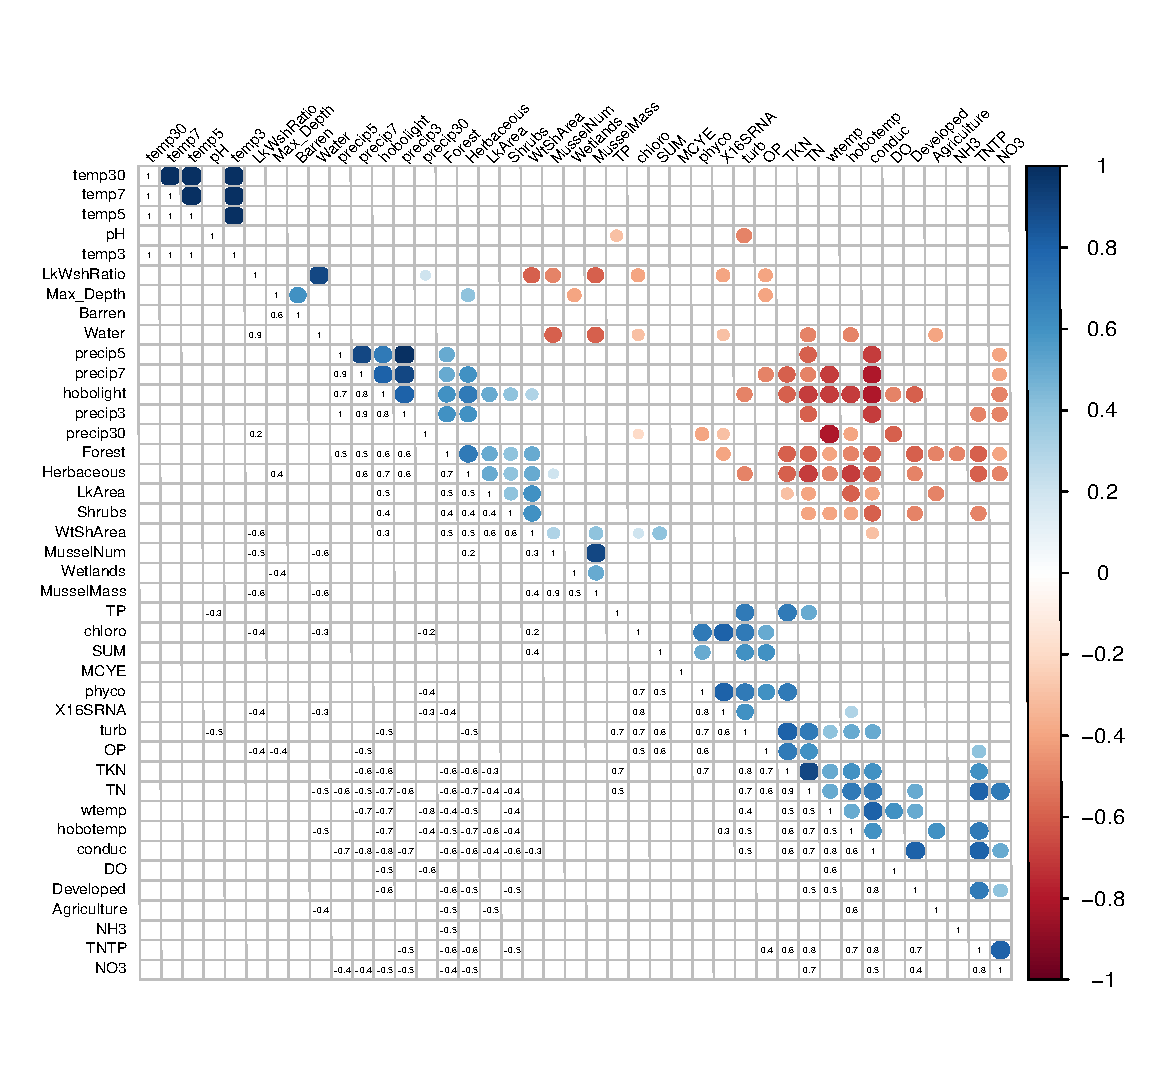
\includegraphics[width=0.9\textwidth]{matrix}
	\vspace*{-15mm}
	\caption{
  Correlation matrix with calculated Pearson coefficient in the lower triangle, and a graphical representation of coefficient value in the upper triangle. Relationships not shown if $\alpha>0.05$. Data matrix was arranged by the angular order of the eigenvectors.}
	\label{matrix}
\end{sidewaysfigure}



%For predicting the \emph{16s rRNA}, we include chloraphyll, turbidity, temperature, lake to watershed ratio, average precipitation 30 days prior and forest land use. A subset analysis was done on the full model including the variables  which was correlated with our response variable. % We found turbidity positively correlated with orthophosphate, total phosphorus, total Kejldahl nitrogen, water temperature, phycocyaninin and chloraphyll. Chlorophyll is positively correlated with \emph{mcye}, phycocyanin, \emph{16S rRNA}, total Kejldahl nitrogen and orthophosphate. Conductance was found to have negative relationship with precipitation. Developed land-use is positively correlated with nitrate+nitrite, total nitrogen and conductance. Watershed area was positive correlated with Zebra mussel mass. Agriculture had a positive relationship with nitrate+nitrite, Forest land-use had negative correlation with total Kejldahl nitrogen, total nitrogen, conductivity, ammonia, nitrate+nitrite and total nitrogen to total phosphorus ratio.Precipitation had negative correlation with total nitrogen, orthophosphate and conductivity.

%Proper way to assess collinearity by linear regression? A caused by B and B caused by A?
In the process of refining our model, $log10$(turbidity) and $log10$(watershed area) were significant predictors when included together ($\beta=0.67$, $F_{{1,26}}=10.93$, $p=0.002$, and $\beta=0.38$, $F_{{1,26}}=9.79$, $p=0.004$). With $log10$(turbidity) as a single predictor variable had a significant effect on total $log10$\gls{mc} ($\beta=0.55$, $F_{{1,27}}=5.90$, $p=0.02$).  $log10$watershed area did explain the residuals of the model with turbidity as a single predictor (see figure \ref{fig:residuals}). The inclusion of $log10$watershed area in our model did have a significant decrease in the residual sum of squares when tested with partial F-test ($p=0.0017$). In a simple linear regression, both turbidity and watershed area as single predictors were significant in predicting $log10$ (\gls{mc}) (see figure \ref{fig:plot2}). Orthophosphate had a positive relationship with $log10$ (\gls{mc}) ($\beta=0.97$, $F_{{1,27}}=5.38$, $p=0.03$), however it was driven by two outlier (see figure \ref{fig:op1}). Removing both outliers, the relationship is still significantly positive ($\beta=1.86$, $F_{{1,25}}=8.77$, $p=0.006$)(see figure \ref{fig:op2}).

\begin{figure}
	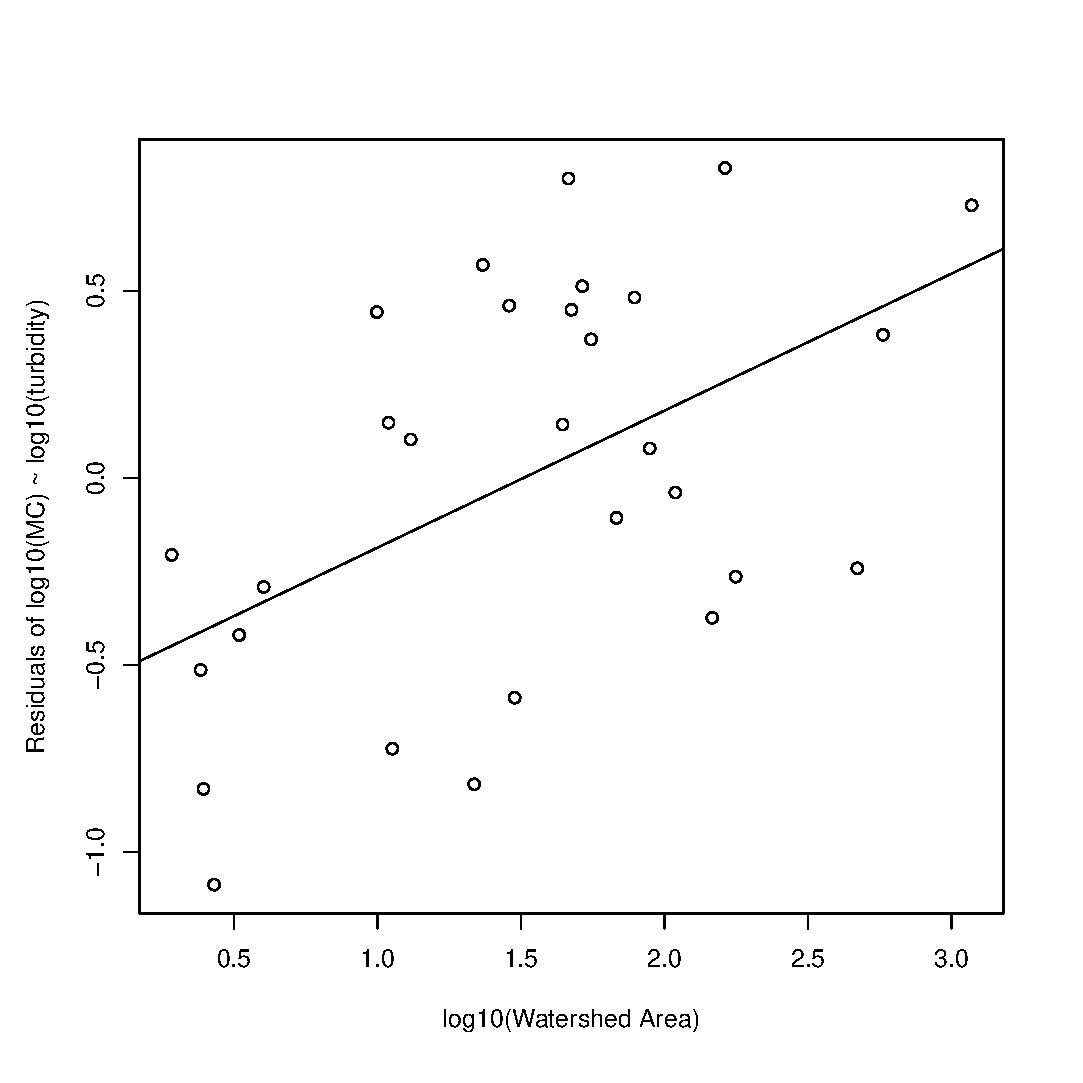
\includegraphics[width=\textwidth]{figures/residual}
	\caption{Residual plot of $log10$(MC) $\sim$ $log10$(turbidity) and $log10$(Watershed area).}
	\label{fig:residuals}
\end{figure}

\begin{figure}
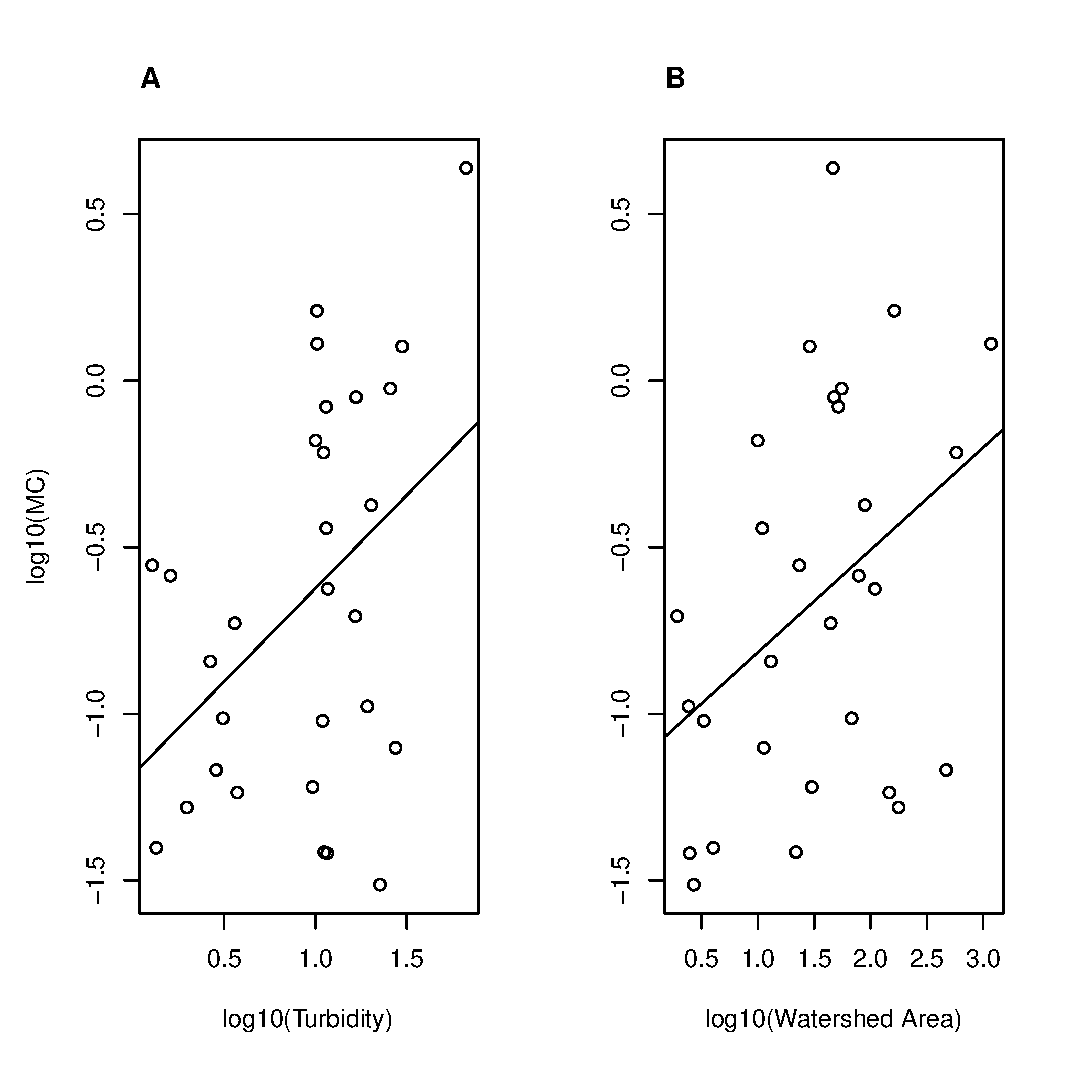
\includegraphics[width=\textwidth, height=11cm]{figures/plot2}
\caption{
(A): Positive relationship between average $log10$(MC) and average $log10$(turb) ($\beta=0.55$, $F_{{1,27}}=5.90$, $p=0.02$)
(B): Positive relationship between average $log10$(MC) and average  $log10$(Watershed Area) ($\beta=0.31$, $F_{{1,27}}=4.88$, $p=0.03$). 
}
\label{fig:plot2}
\end{figure}



\begin{figure}[p]
	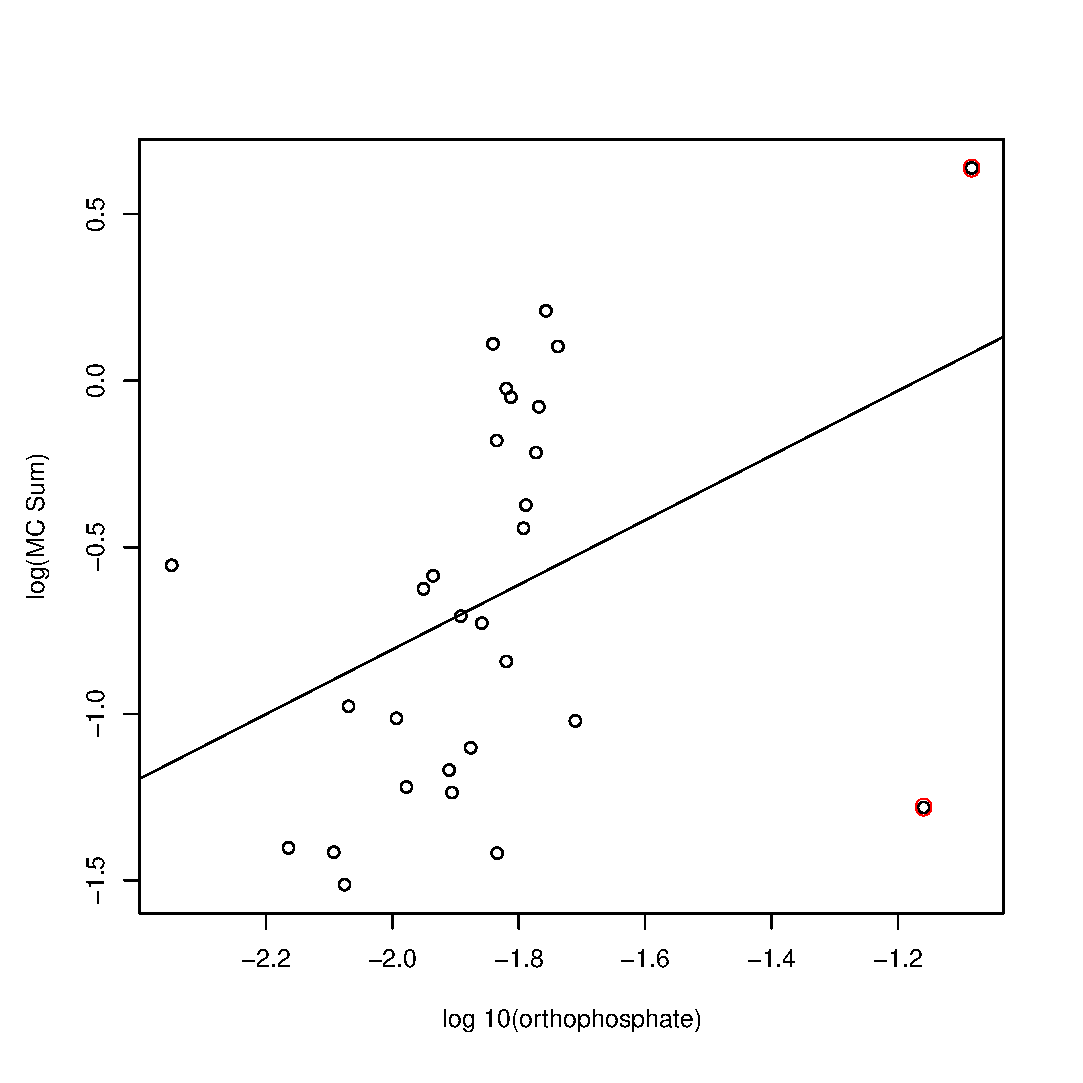
\includegraphics[width=\textwidth]{op1}
	\caption{Positive relationship between average $log10$(MC) and average $log10$(Orthophosphate)($\beta=0.97$, $F_{{1,27}}=5.38$, $p=0.03$). Outliers are identified in red. }
	\label{fig:op1}
\end{figure}

\begin{figure}[p]
	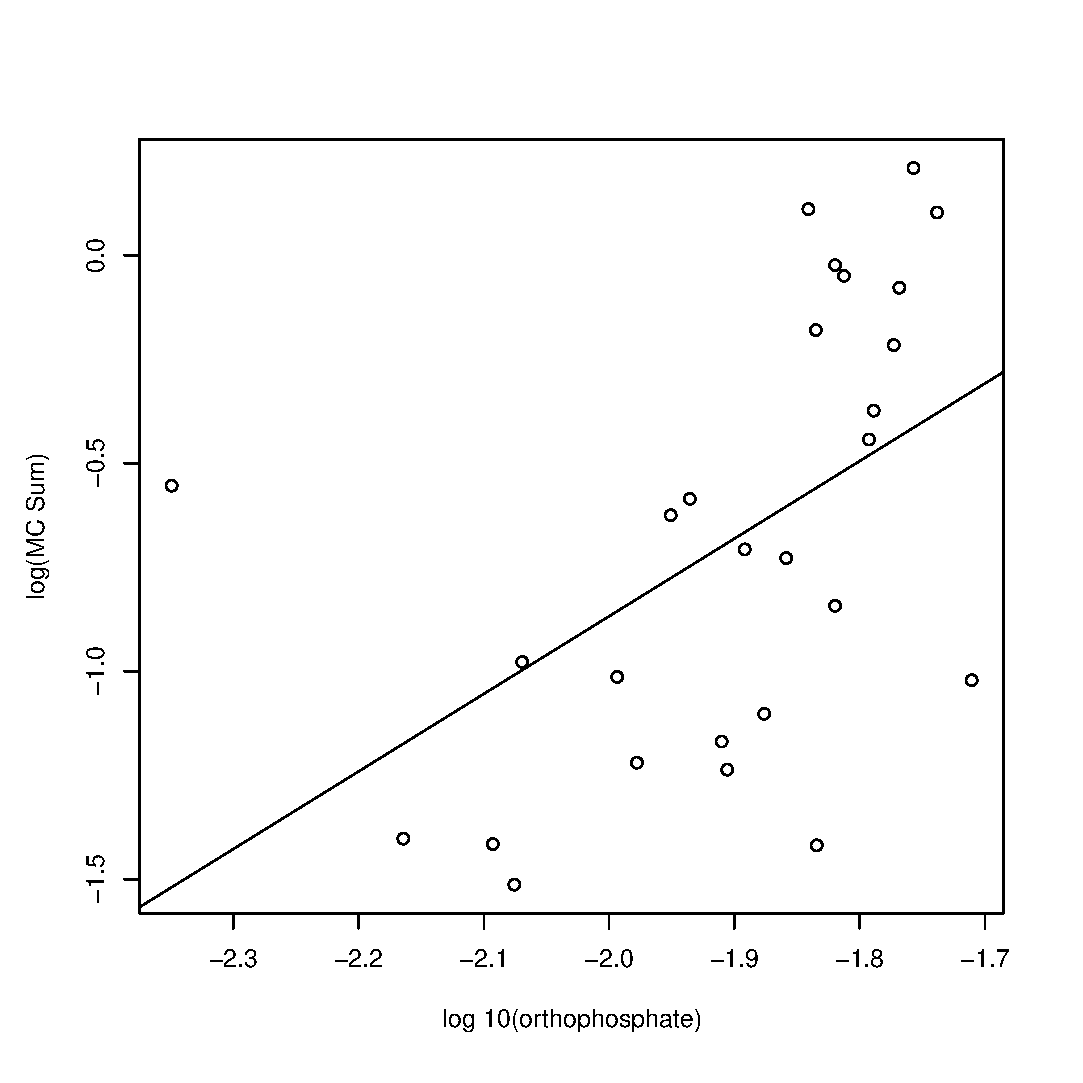
\includegraphics[width=\textwidth]{op2}
	\caption{Positive relationship between average $log10$(MC) and average $log10$(Orthophosphate) with outliers removes ($\beta=1.86$, $F_{{1,25}}=8.77$, $p=0.006$) }
	\label{fig:op2}
\end{figure}


%With our model selection from our data, $log10$(Orthophosphate) was shown to be positively correlated with $log10$(turbidity) from our exploratory analysis, with a simple linear regression analysis, the relationship is slightly significant ($\beta=0.57$, $F_{{1,26}}=3.13$, $p=0.08$). The regression did have outliers, with the two data points removed the relationship is significant ($\beta=0.17$, $F_{{1,25}}$, $p=0.01$) (see \ref{fig:plot1}). We avoid including either $log10$(orthophosphate) or $log10$(turbidity) in our models together.
%All other variables did not have any significant correlations with eachother.
%From backward stepwise regression, eliminated  contained 3 variables, orthophosphate, max depth and turbidity.
%With $log10$(\emph{mcyE}) as a single predictor in a linear mixed model shown to have a significant relationship with $log10$(MC), however we are missing data from July ($N=91$) which does not allow us to use the full dataset ($\beta=0.15$, $F_{{1,72}}$, $p=0.002$).

%We found $log10$(turbidity) as the best single predictor. The relationship was significant with predicting $log10$(MC) concentration in a linear mixed-effect model ($\beta=0.55$, $F_{{1,27}}=5.90$, $p=0.02$) (see \ref{fig:plot2}). However, with $log10$(orthophosphate) as a single predictor the relationship is almost significant ($\beta=0.35$, $F_{{1,26}}=3.13$, $p=0.07$) (see \ref{fig:plot2}).  The best model for predicting MC is turbidity as the sole predictor. Adding additional predictors did not significantly improve the model.


%For predicting the $log10$(\emph{16s rRNA}) gene copies, chloraphyll, agriculture land-use and average temperature 3 and 30 days prior to sampling and precipitation 5 days before sampling were investigated for building our model (see figure \ref{subset2}). Precipitation and temperature data did not have significant relationship and was eliminated from the model. Agriculture percent land-use found to be the best predictor for \emph{16s rRNA} ($\beta=0.70$, $F_{{1,26}}=5.10$, $p=0.03$)(figure \ref{fig:agriculture})

\section{\emph{A Priori} Hypothesis Test}

In my hypothesis, I expected developed land-use percentage to have a positive influence on MC concentrations. Developed land-use percentage plotted had a slight positive effect with $log10$(MC) concentration , however the relationship was not significant  ($\beta=0.59$, $F_{{1,27}}=1.75$ , $p=0.20$)(see figure \ref{fig:developed}). There were no significant relationship with developed land-use percentage in predicting $log10$(\emph{16s rRNA}) gene copies ($\beta=0.48$, $F_{{1,25}}=1.75$ , $p=0.27$). Developed land-use did not have a significant relationship in predicting orthophosphate ($\beta=0.37$, $F_{{1,27}}=2.60$ , $p=0.11$), ammonia ($\beta=0.33$, $F_{{1,27}}=0.75$ , $p=0.39$), total phosphorus  ($\beta=0.33$, $F_{{1,27}}=0.75$ , $p=0.39$) and total nitrogen ($\beta=0.48$, $F_{{1,25}}=1.75$ , $p=0.27$) However, developed land-use had a positive significant relationship with log10(nitrate+nitrite) ($\beta=0.75$, $F_{{1,27}}=1.08$, $p=0.018$). 

Forest land-use percentage had a significant negative relationship with $log10$(\emph{16s rRNA}) gene copies ($\beta=-1.42$, $F_{{1,25}}=7.08$, $p=0.013$)(see figure \ref{fig:forest}). However, forest land use did not have a significant effect on $log10$(MC) concentrations ($\beta=-0.34$, $F_{{1,26}}=0.32$, $p=0.57$).

With the surveyed lakes, 17 out of 29 had Zebra mussels found in the month of October. The average MC concentrations with  of Zebra mussles present was 0.568 $\mu$g/L, and absent with 0.305 $\mu$g/L. Using a two sample Student's t-test, we fail to reject the null where difference of the mean is greater than 0 ($t=1.14$, $df=107$, $p=0.13$). We also did not find any significant relationship with the mussel counts and mass with predicting MC concentration.




%\begin{figure}[!ht]
%	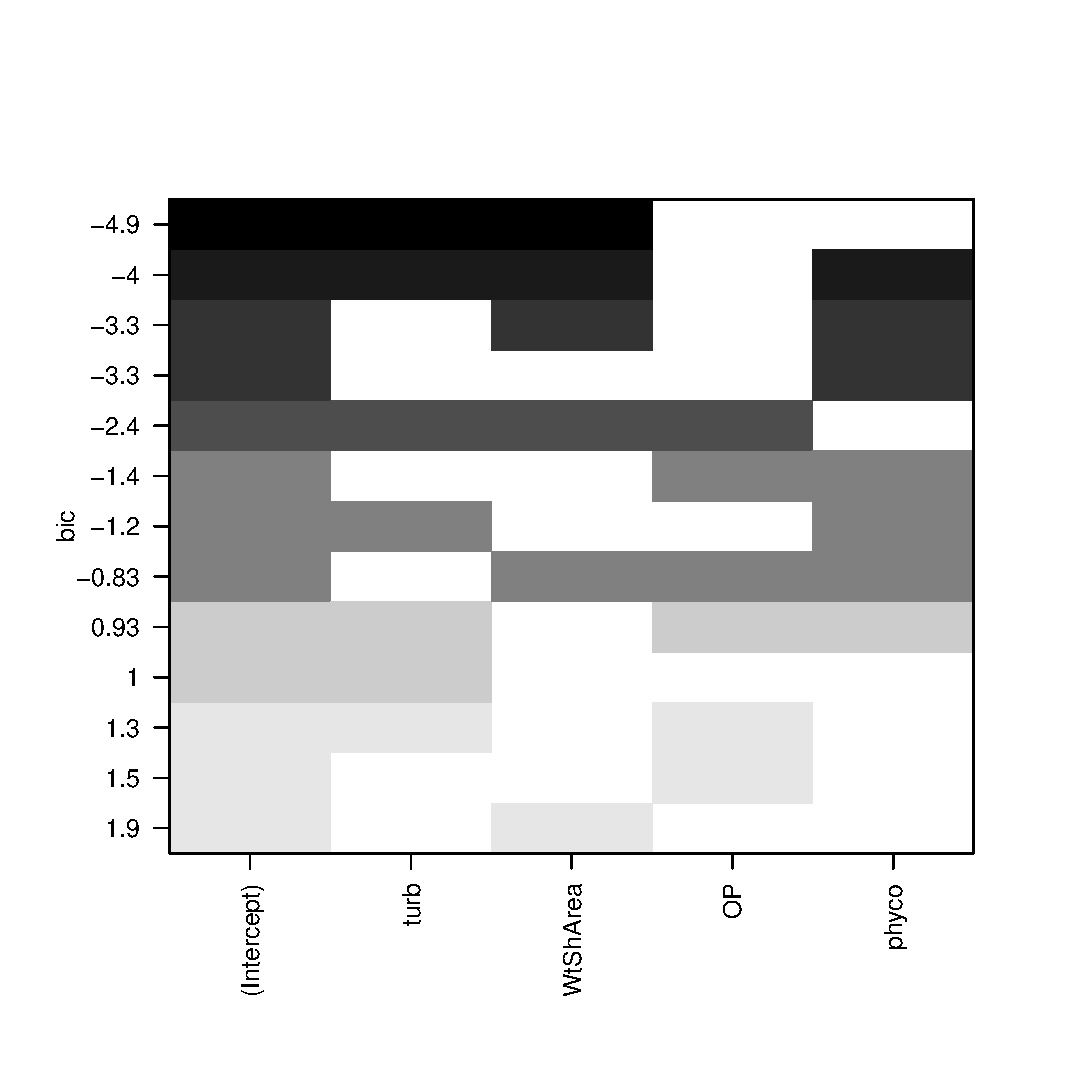
\includegraphics[ width=\textwidth]{subset2}
%  	\vspace*{-15mm}
%	\caption{Subset regression analysis with MC Sum from LC-MS/MS as response variable. Each row is a model. Variable is included in the model it is represented as a black rectangle. The BIC is plotted on the y axis where the lowest value is higher up on the axis.}
%	\label{fig:subset}
%\end{figure}

%\begin{figure}[!ht]
%  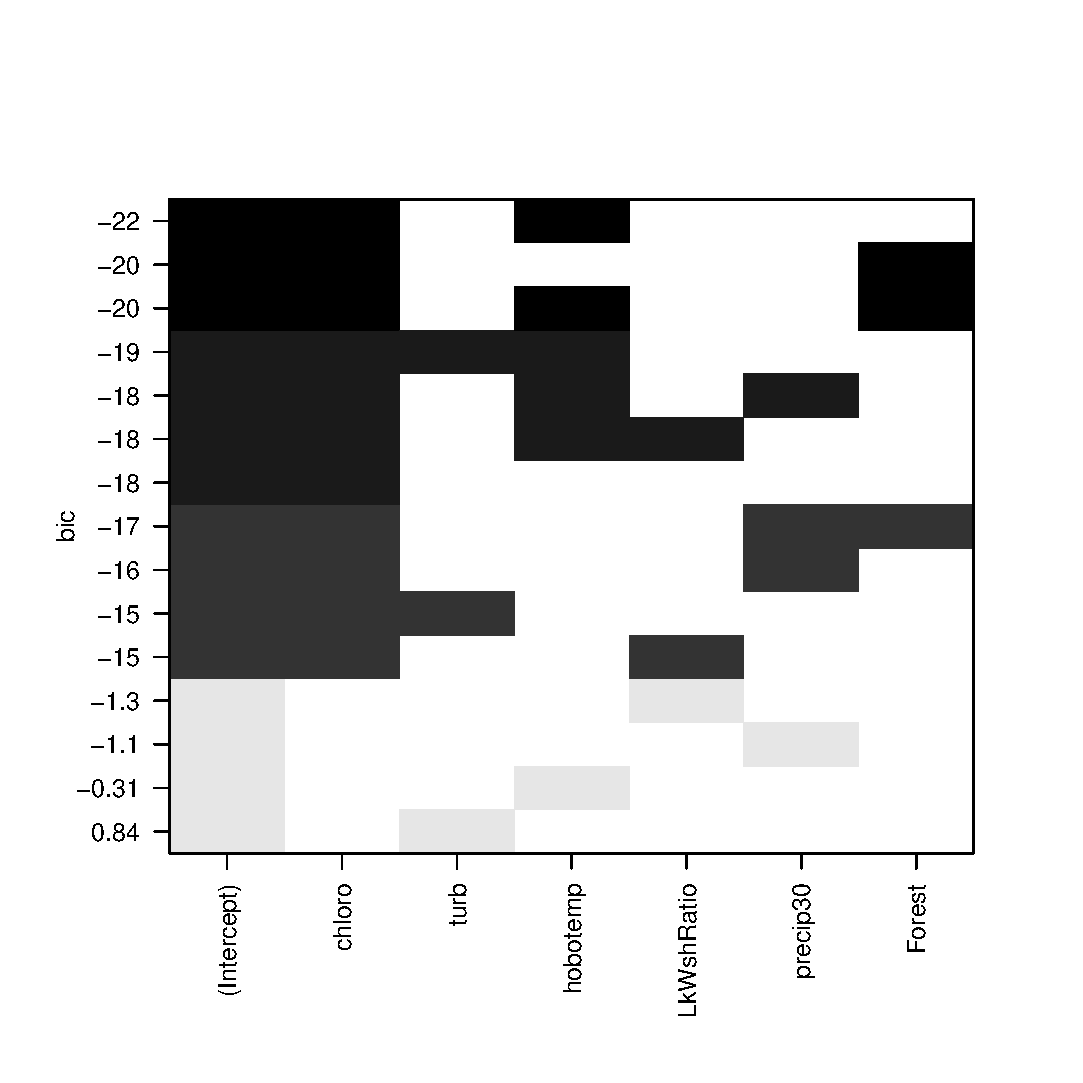
\includegraphics[ width=\textwidth]{subset3}
%  \caption{Best Subset: \emph{16s rRNA} Gene copies as response variable}
%  \label{fig:subset2}
%\end{figure}

%\begin{figure} 
%	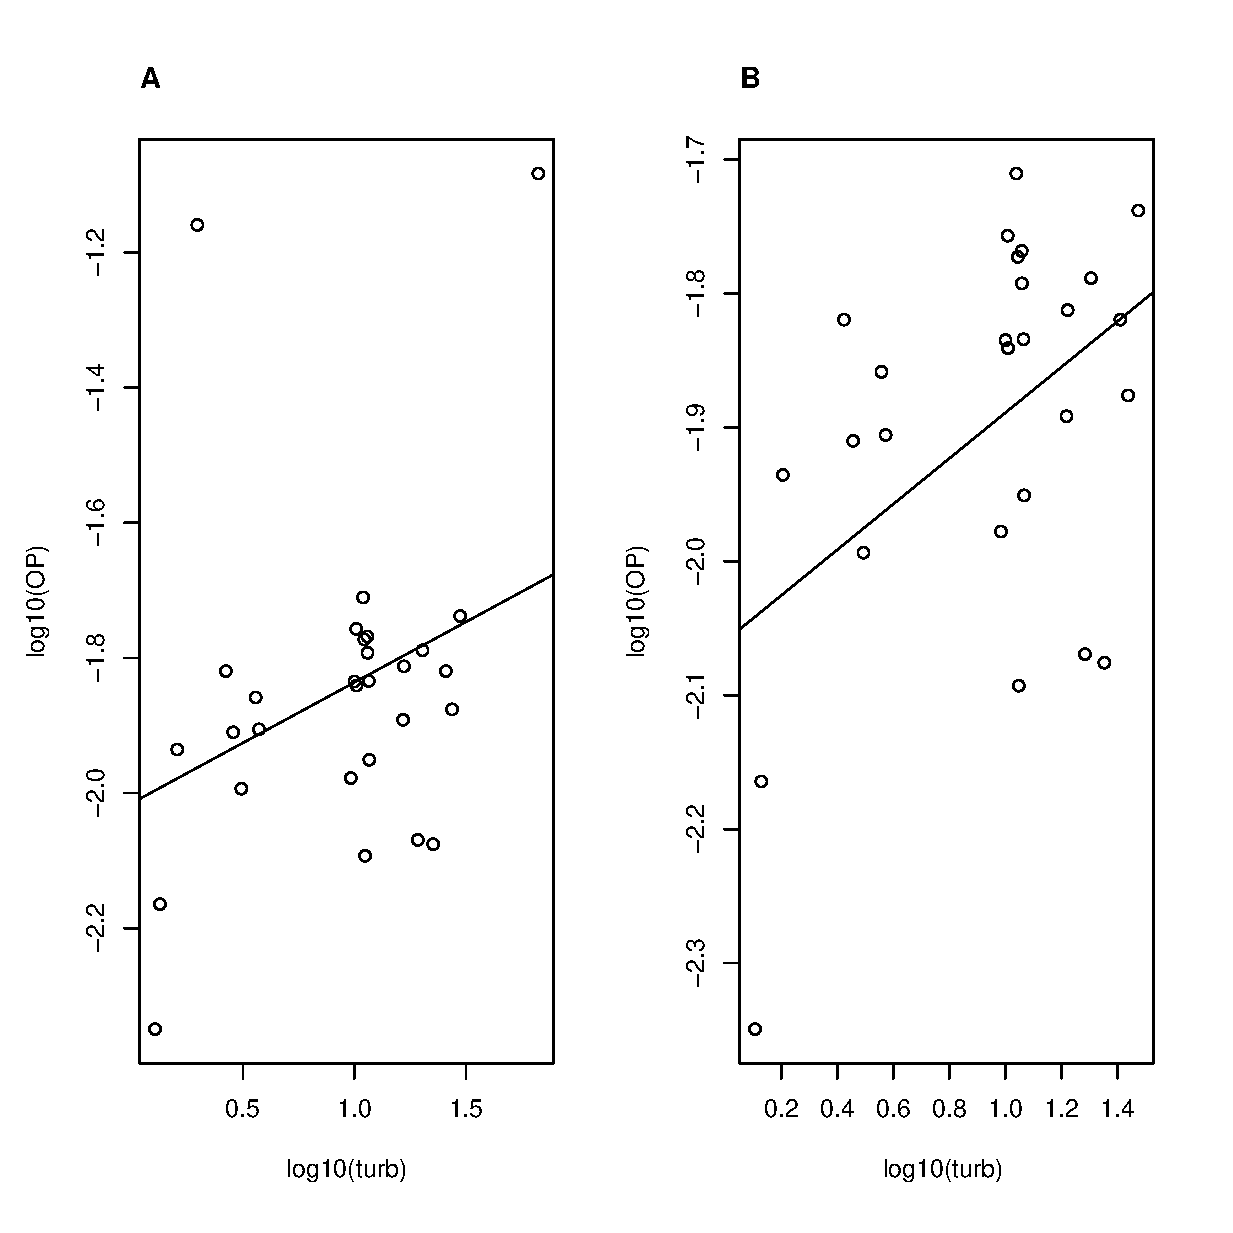
\includegraphics[width=\textwidth, height=11cm]{figures/plot1}
%	\caption{
%(A): Positive relationship with average $log10$(OP) with average $log10(turb)$ ($\beta=0.57$, $F_{{1,26}}=3.13$, $p=0.08$).
%(B): With two outliers removed, the relationship between $log10(OP)$ and $log10(turb)$ was signifigant  ($\beta=0.17$, $F_{{1,25}}$, $p=0.01$).
%}
%	\label{fig:plot1}
%\end{figure}



\begin{figure}[p]
	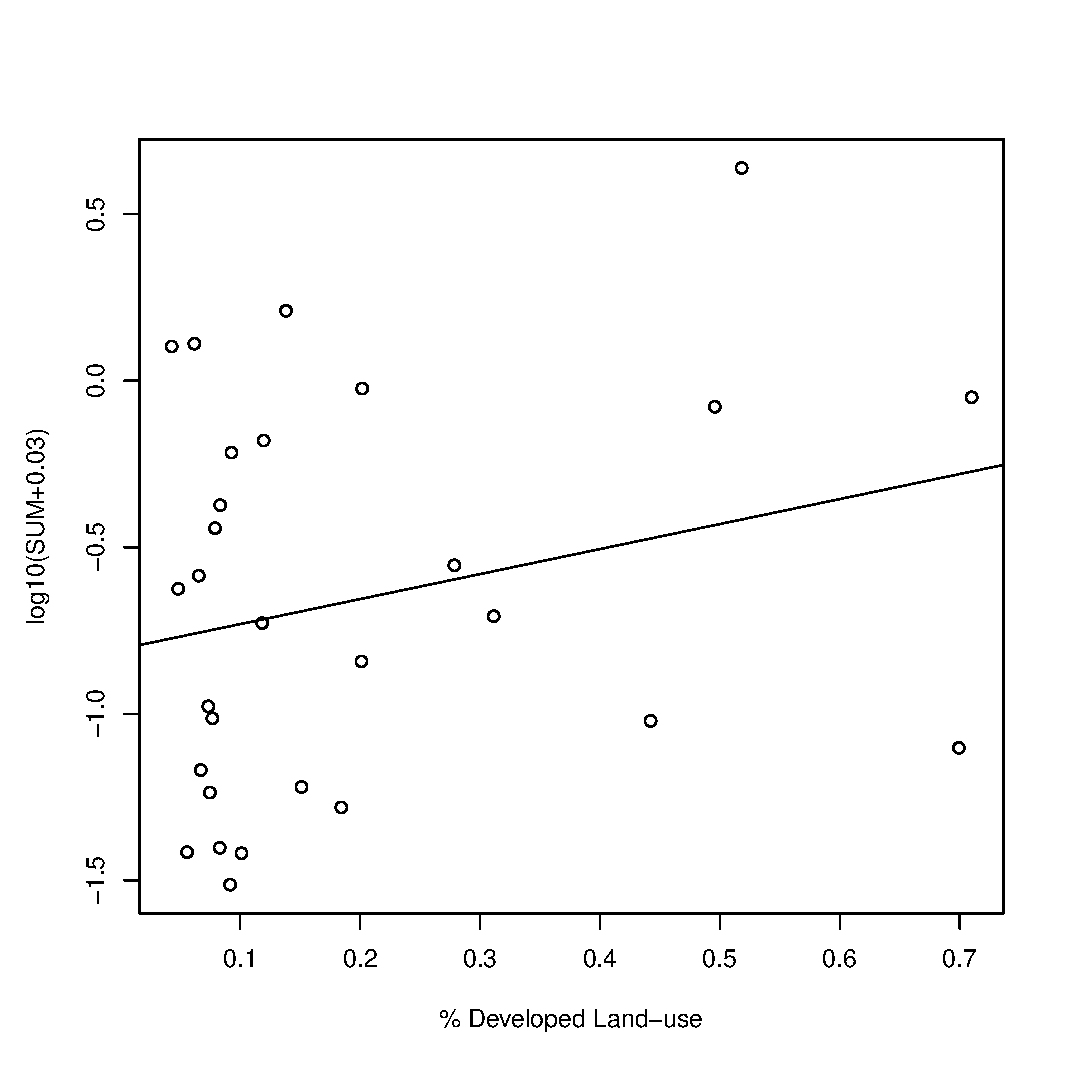
\includegraphics[width=\textwidth]{figures/developed}
	\caption{
A slight positive relationship between $log10(MC)$ and developed land use. ($\beta=-0.59$, $F_{{1,27}}=1.75$, $p=0.20$)
}
	\label{fig:developed}
\end{figure}

\begin{figure}[p]
	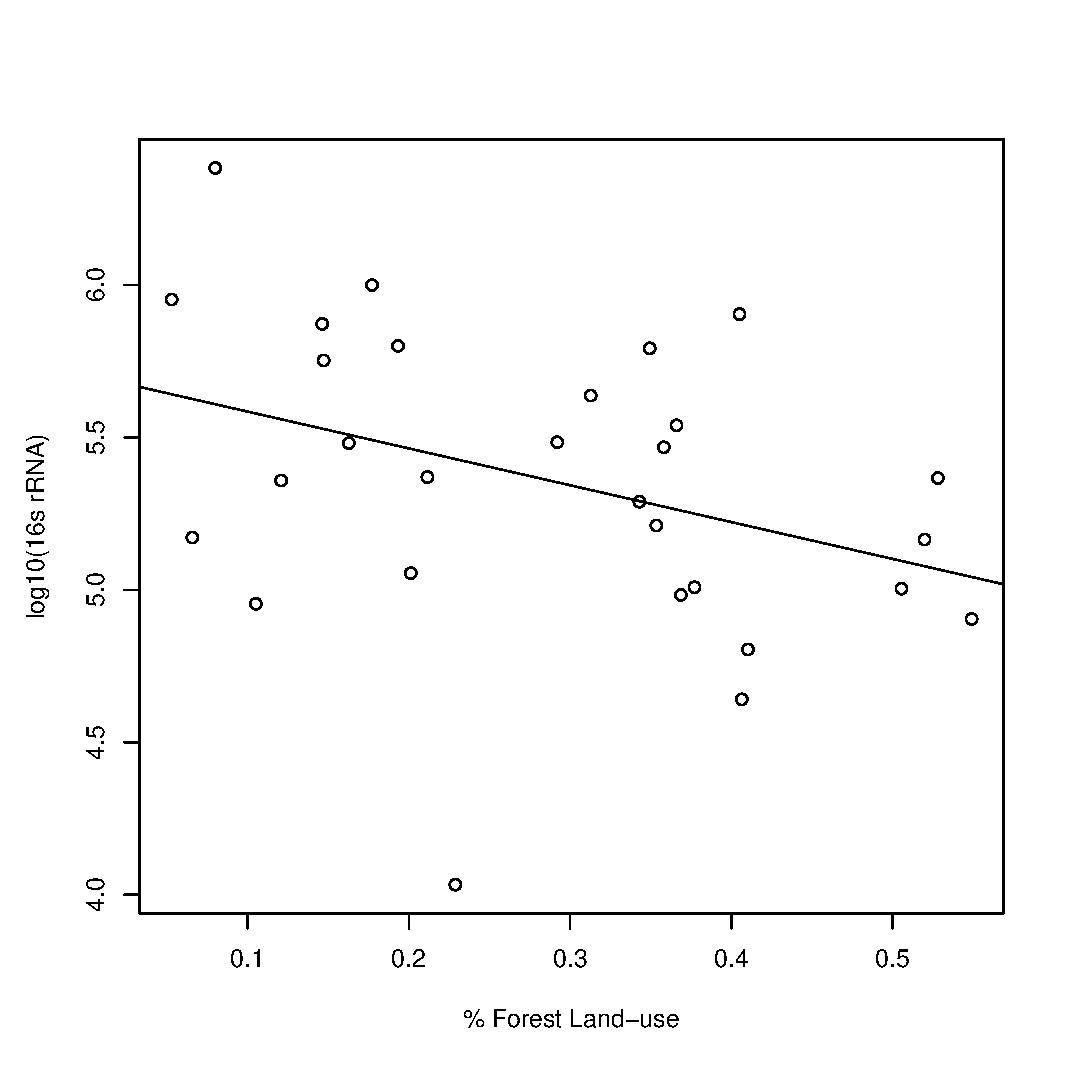
\includegraphics[width=\textwidth]{figures/forest}
	\caption{
A negative relationship between $log10(MC)$ and forest land use. ($\beta=-1.42$, $F_{{1,25}}=7.08$, $p=0.013$)
}
	\label{fig:forest}
\end{figure}




\begin{figure}[p]
	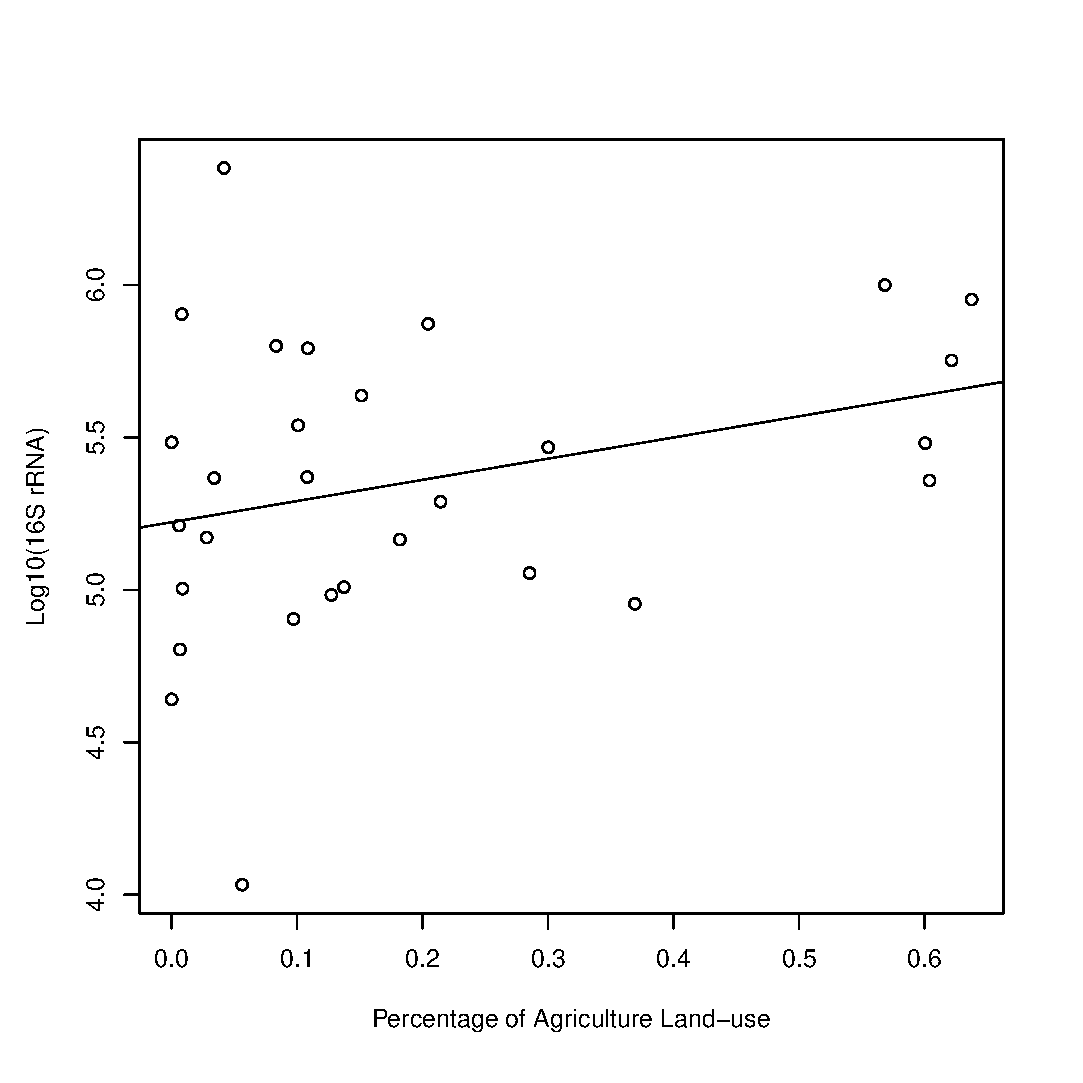
\includegraphics[width=\textwidth]{figures/Agriculture}
	\caption{
Positive relationship between percent agriculture land-use and $log10$(\emph{16s rRNA}) ($\beta=0.70$, $F_{{1,26}}=5.10$, $p=0.03$)
}
	\label{fig:agriculture}
\end{figure}



\section{Discussions}

In my first hypothesis, I tested if disturbance from developed land is associated with \gls{hab} and if it has an affect on nutrient concentration.  From our data, we did not find a significant relationship between developed land use and MC concentrations or \emph{16s rRNA}. However, we did find developed land use having some effect with nitrate+nitrite. We did observe some relationship between land use and nutrient concentrations from the correlation matrix, but the associations were not significant.
Much of the southern lakes were vastly dominated by developed land such as Belleville, Ore, Brighton, Ford and Bogie Lake. 

Identifying turbidity could help predicting at risk lakes. Turbidity can be an indicator of other parameters such as the stability of the riparian zone and urbanization. Turbidity was found to also a good predictor with cyanobacteria biomass, but also found \gls{mc} more abundant in natural lakes comparatively to human-made \cite{taranu_predicting_2017}.  


Orthophosphate was shown to be significant in predicting \gls{lcmsms}. There were two outliers which was from Brighton and Stony Lake. Brighton Lake had high levels of \gls{mc} and orthophosphate. Stony lake had high levels of orthophosphate but had low levels of \gls{mc}. This may due to an instance where the surface water level dropped 4-6ft in October 2017. This may have given the result of orthophosphate to be higher than normal. With both removed, the relationship was still significant with \gls{mc}. However, orthophosphate did not predict \emph{16s rRNA} gene copies ($\beta=0.61$, $F_{{1,27}}=2.92$, $p=0.10$).
%Wixom lake is very unique, it has the largest watershed amongst all our surveyed lake and has visually one of the largest extent
In other studies, many have emphasized nutrients to be a limiting factor in \gls{hab} growth.  which is long believed to be a useful parameter to measure. Cultured study done by Hee-Mock Oh et al. found relationship the growth rate limited by the ratio of nitrogen to phosphorus ratio \cite{oh_microcystin_2000}. In our survey, we did not observe total nitrogen to total phosphorus to have an association. However, mesocosm experiments do not necessary translate to real world scenarios, but do provide some insight. Orthophosphorus does seem to be a good indicator for our survey. 

Comparing the average results from SPATT to the grab sample, we identified a major difference (see \ref{fig:spattbox}). When average concentration of MC from SPATT and grab sample is ordered by latitude, we found the relative magnitude of MC to be higher found in the upper latitude of Michigan compared to regular grab sample. In our grab sample, Brighton, Pontiac, Wixom Lake and Lake Cadillac had high average of MC with notable \gls{hab}, however Brighton and Pontiac Lake were not detected relatively. The SPATT also detected relatively high amounts of \gls{mc} which our grab samples did not detect, in particular with Lake Paradise, Wixom and Cadillac. 

The results from SPATT seemed to suggest the lakes we found to have low MC from our grab sample missed other \gls{hab}. When lakes were ordered by latitude, it also suggest lakes found in the upper latitude of Michigan may have had higher frequency of \gls{hab} that we missed. Although we speculate some other factors that explains the higher magnitude of MC. We started to observe  some biofilm to accumulate on the SPATT bags. The biofilm was more notable in lakes that had significant blooms such as Brighton, Pontiac, and Wixom Lake. Initially we did not expect this would effect the capacity of the SPATT, but this data may suggest this. Dispatching the SPATT bags more often could prevent biofilm to encase and clog the Nitex mesh bag. Another approach to prevent biofilm to accumulate is to wrap each SPATT bags in copper wire to prevent growth but still allow toxins to adsorb onto the resin. Another factor that could possibly be the issue is the fact that extracellular cyanotoxins is degraded when exposed to sunlight. In our grab samples, we would be measuring low levels of cyanotoxins, but the SPATTs would be measuring the accumulation of extracellular cyanotoxins. This could also be creating the discrepancy between the SPATT and the grab results. 



\begin{figure}[p]
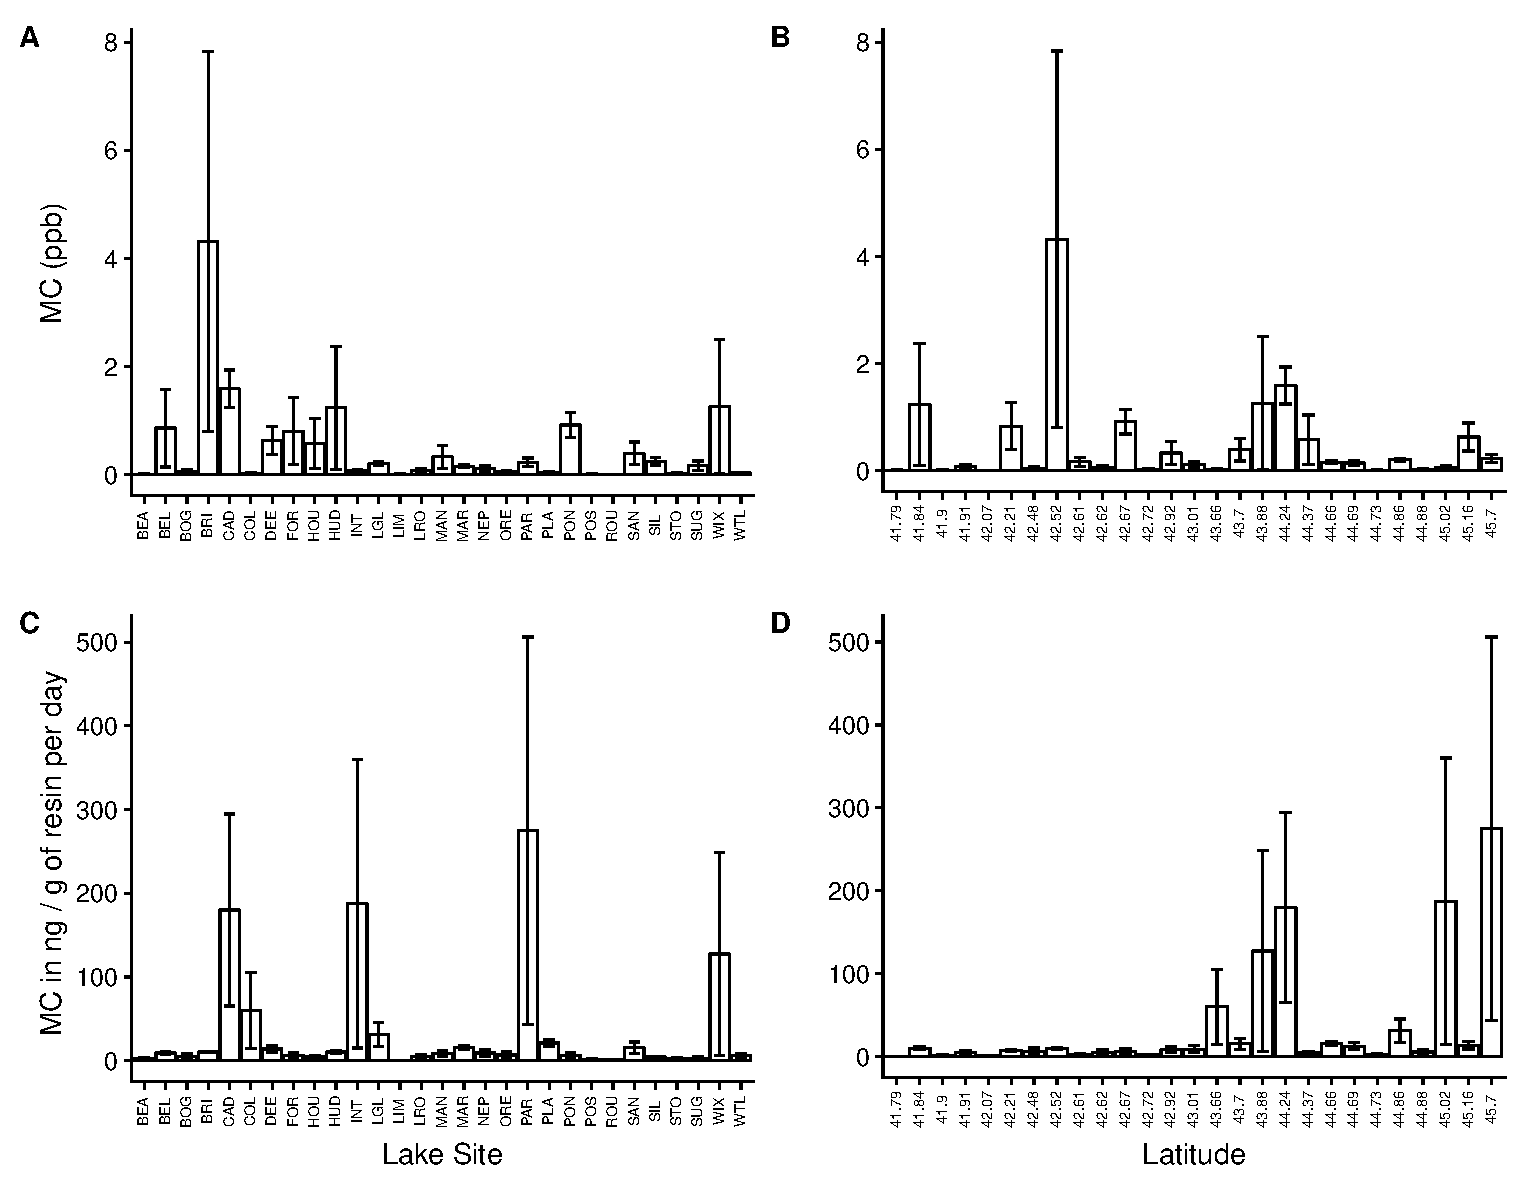
\includegraphics[width=\textwidth]{figures/spatttboxplotlake}
\caption{
Microcystin measured from SPATTS compared to grab sample: and Grab Samples. Average concentration of MC are plotted as bar graphs. Microcystin concentrations analyzed from grab sample are shown in figure (A) arranged by each lake and (B) arranged by latitude. Microcystin concentrations analyzed from SPATT samples are shown in figure (C) arranged by each lake and figure (D) arranged by latitude
}
\label{fig:spattbox}
\end{figure}



\gls{mc} is a widespread source water and recreational water problem. Analysis of MC is complicated by the large number of congners. \gls{lcmsms} is limited to known congeners with commercial sources. The ADDA ELISA is not congener independent \cite{he_varied_2017}. When \gls{lcmsms} and ELISA are compared in our grab samples, there are discprenancies between the two. Analysis from ELISA tends to be report higher values than \gls{lcmsms}. The difference is more apparent in the month of September and October, where the difference can be quite large (see figure \ref{fig:compare}). The ELISA generally presents a higher result than \gls{lcmsms}. This is in part due to the detection limit and reportable limits being much higher for the ELISA, 0.15 and 0.1 $\mu$g/L. However, our analysis in the month of August had good agreement between \gls{lcmsms} and ELISA. 

We ran a correlation matrix analysis on the \gls{mc} variants and found congeners with arginine (R) containing groups to be correlated with all other congener with arginine groups (see figure \ref{fig:congenermatrix}). \gls{mcla} did not correlate with no other congener. We also tested if the discrepancy between the ELISA and \gls{lcmsms} by taking their difference and also including in the correlation matrix but did not find any associations. 

\begin{figure}[p]
	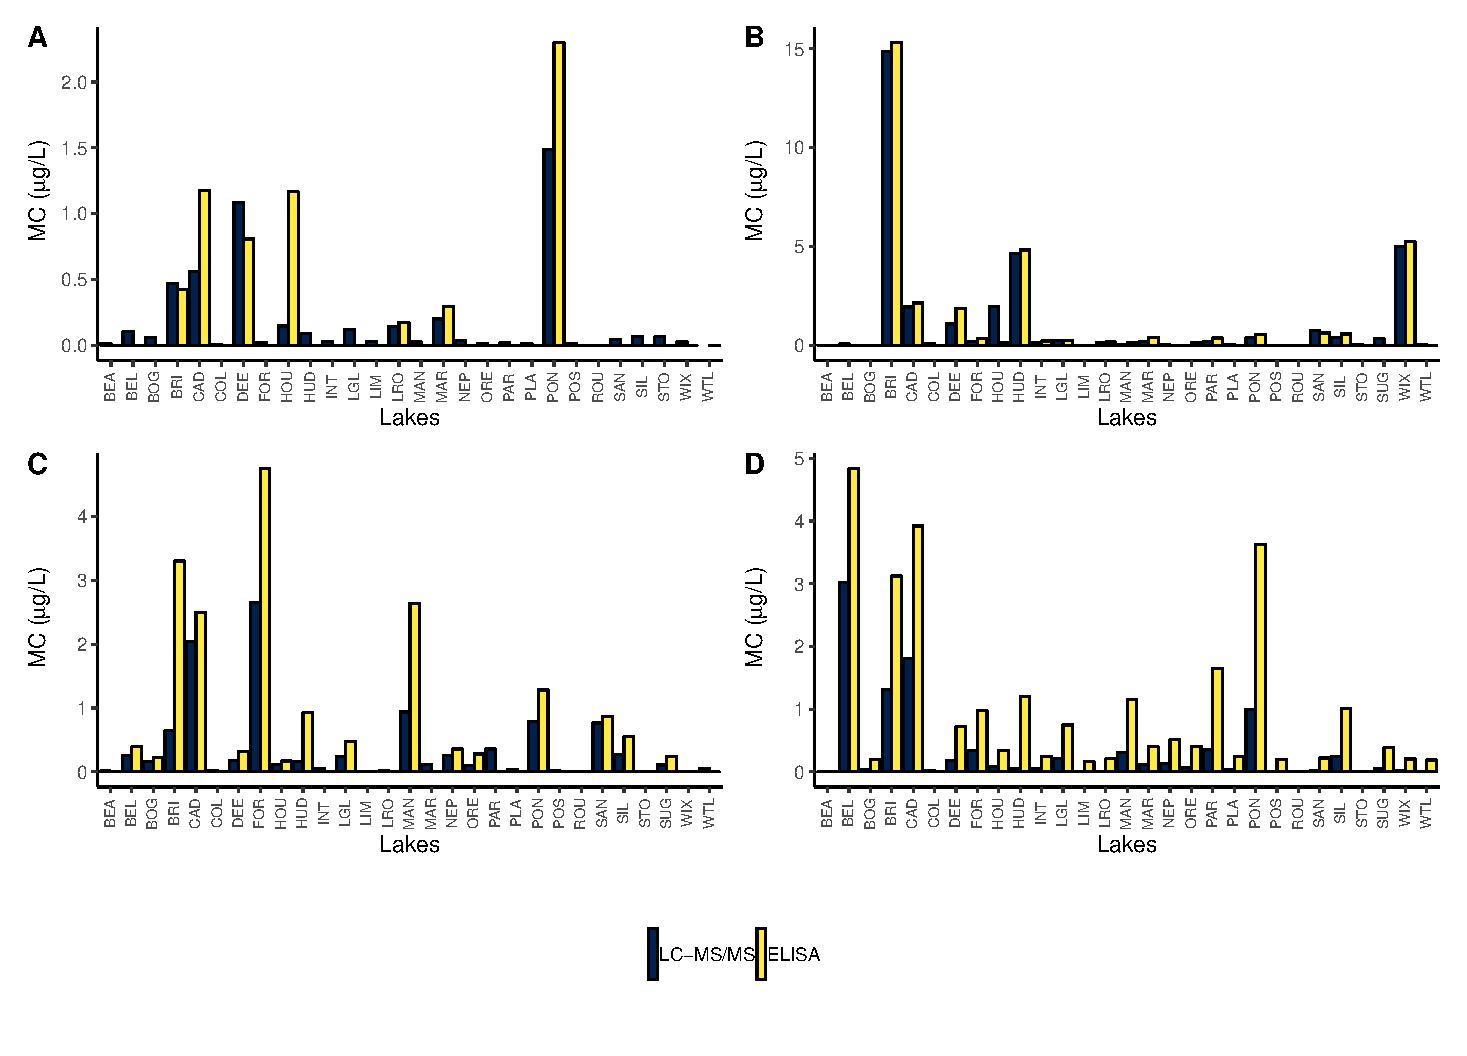
\includegraphics[width=\textwidth]{figures/compare}
	\caption{Barplots of MC analyzed by LC-MS/MS and ELISA. Concentrations are shown for the month of: (A) July, (B) August, (C) September and (D) October}
	\label{fig:compare}
\end{figure}



\begin{figure}[p]
	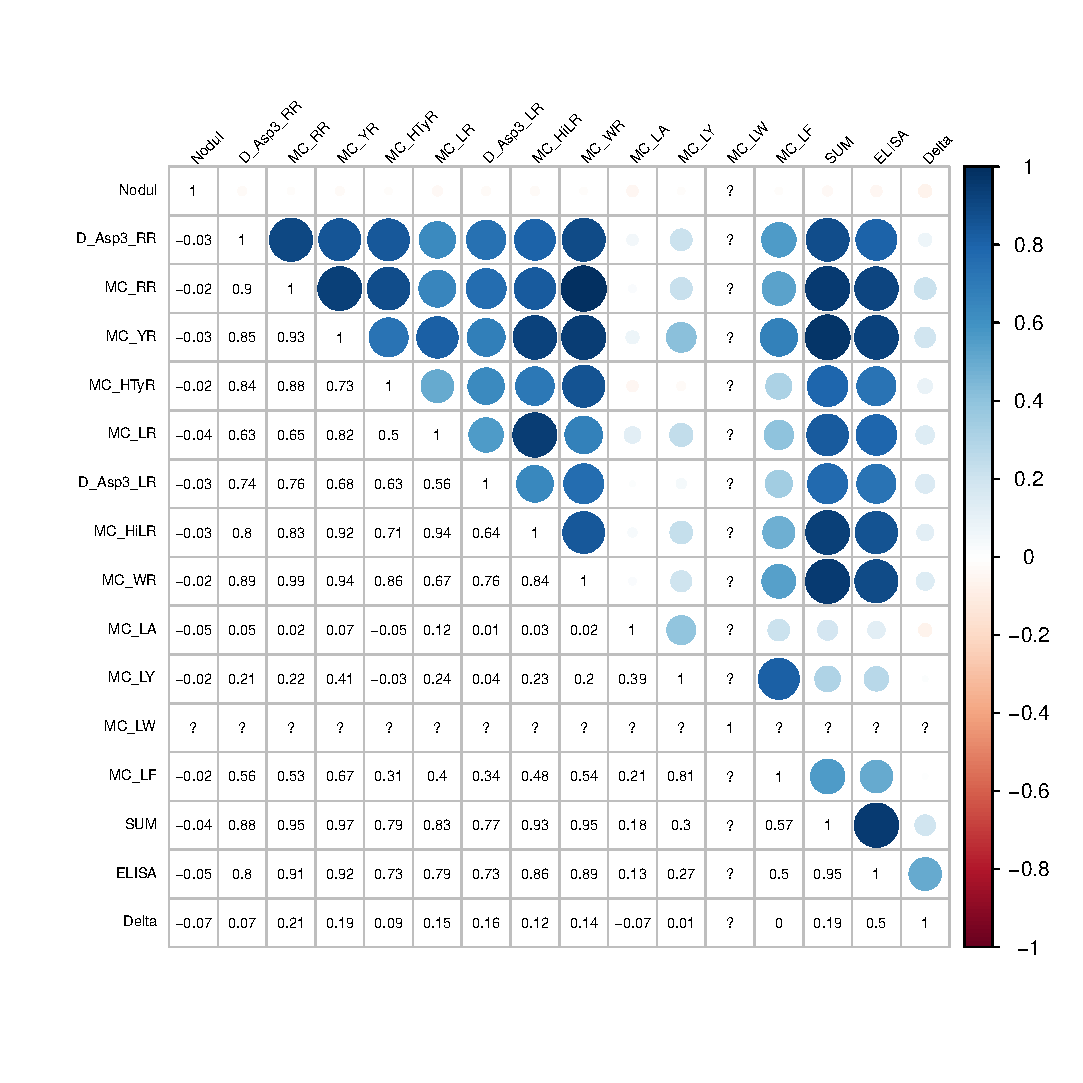
\includegraphics[width=\textwidth]{figures/congener_matrix}
	\caption{Correlation matrix of MC congeners}
	\label{fig:congenermatrix}
\end{figure}



%Dissolved oxygen averaged around 12.98$\pm$20.8 mg/L of \ch{O2}.

% FORMS OF NUTRIENTS TODO revise this, expand it

% revise this and put more work into this TODO
% Cyanobacteria are versatile as they can acquire nutrients under extreme conditions. The diversity of different genera or species needs to be accounted as different species can out compete the other. 

%They can utilize a process called quorom sensing which they coordinate with each other by using a signaling hormone acylated homoserine lactones \cite{van_mooy_quorum_2012}. They also can create a network of cells which work together as a unit, often as seen as a layer of green goo floating on top of water. Environmental factors that could trigger this response may need to be accessed as this could give certian toxin producing genera's a competitive advantage. 

% There are very robust organisms, as some can change their buoyancy by modulating the intracellular gas vesicles gives them a competitive advantage over other species for seeking light \cite{feng_how_2018}.\emph{Microcystis} can form a complex colony made by a mucilage structure which can be bouyant due to high concentration of dissolved oxygen \cite{xiao_colony_2018}. % TODO expand how co2 gets pumped into gas vesicles
% Most of the cyanotoxin are intracellular, however with increase turbulence from wind and precipitation can release more toxins due to cell lysis either from cell apoptosis or from mechanical abruption which release \cite{rohrlack_fate_2007}. % TODO cyanophages, viruses 


% Forest has negative correlation with NUTRIENTS

%A study in South Korea found 3-week lagged water temperature,dissolved oxygen and pH with to correlate with each other in their models \cite{ahn_evaluation_2011}.

%Growing cyanobacteria measurements taken at the same time . Their is an assumption being made.

%Total nitrogen was found to explain the variance of MC concentrations \cite{taranu_predicting_2017}.

%Man-made lakes are found to be twice as higher concentrations in cylindrospermonsin \cite{loftin_cyanotoxins_2016}.


%Low-nutrient lakes can still exhibit blooms.
 %This can complicate our model as this is not accounted for.

%QPCR results as a response variable comes with complication as this does not distinguish alive or dead cyanobacteria.




%Water sampling for nutrient is difficult. Time series data, nutrient dynamic. Continuous measurements  water data would be best, but for a large survey its almost impractical. Other organisms compete with these common nutrients. Aquatic macrophytes largely acquire dissolved phosphorus. Time between sampling the lake at the peak of the bloom and the flush of nutrient inputs can be lagged, and most likely different depending on each lakes morphology. Biological properties are not necessarily linear. One thing to consider here is the sampling frequency. We sampled once a month for four months, which gives four sampling results for each lake. This may not explain everything about each lake.

% How pH and DO has an influence on nutrient availability





